\usetikzlibrary{arrows.meta, calc}


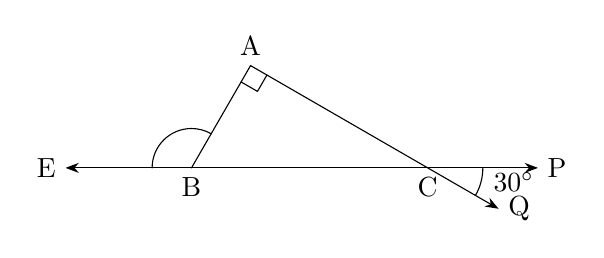
\begin{tikzpicture}[>=Stealth, line join=round, line cap=round, scale=2]
    % --- COORDINATES ---
    % Origin at B, C placed such that angle ABC is 60 degrees
    \coordinate (B) at (0, 0);
    \coordinate (C) at (1.5, 0);
    
    % A is calculated so that angle BAC = 90 and angle ACB = 30
    % For BC = 1.5, AB = 1.5 * cos(60) = 0.75
    \coordinate (A) at ({0.75*cos(60)}, {0.75*sin(60)});
    
    % External points on the lines
    \coordinate (E) at (-0.8, 0);
    \coordinate (P) at (2.2, 0);
    
    % Q is an extension of the ray starting from A through C
    \coordinate (Q) at ($(A)!1.4!(C)$);

    % --- DRAWING ---
    % Draw the horizontal line EP with arrows
    \draw[<->] (E) -- (P);
    
    % Draw the line segment AB
    \draw (B) -- (A);
    
    % Draw the ray starting from A, through C, ending at Q with an arrow
    \draw[->] (A) -- (Q);

    % --- ANGLE MARKS ---
    % 1. Right angle at A
    % The right angle symbol is a square aligned with segments AB and AC
    \begin{scope}[shift={(A)}, rotate=-30]
        \draw (0,-0.12) -- (0.12,-0.12) -- (0.12,0);
    \end{scope}

    % 2. Arc for the exterior angle ABE
    % Arc starts from direction 180 (towards E) to direction 60 (towards A)
    \draw (B) ++(180:0.25) arc (180:60:0.25);

    % 3. Arc and label for the exterior angle PCQ (30 degrees)
    % Arc starts from direction 0 (towards P) to direction -30 (towards Q)
    \draw (C) ++(0:0.35) arc (0:-30:0.35) node[midway, right, xshift=1pt] {$30^\circ$};

    % --- LABELS ---
    \node[above] at (A) {A};
    \node[below] at (B) {B};
    \node[below] at (C) {C};
    \node[left] at (E) {E};
    \node[right] at (P) {P};
    \node[right] at (Q) {Q};

\end{tikzpicture}